\documentclass[11pt,twocolumn]{article}
\usepackage[margin=0.58in]{geometry}
\usepackage{graphicx}
\usepackage{amsmath}
\usepackage{amssymb}
\usepackage{booktabs}
\usepackage{array}
\usepackage{caption}
\usepackage{enumitem}
\usepackage{hyperref}
\usepackage{titlesec}
\usepackage{xcolor}
\setlength{\parindent}{0pt}
\setlength{\parskip}{3pt}
\setlength{\columnsep}{0.22in}
\setlist[itemize]{leftmargin=*, topsep=1pt, itemsep=1pt, parsep=0pt}
\titlespacing*{\section}{0pt}{5pt}{2pt}
\titleformat{\section}{\large\bfseries}{}{0pt}{}
\captionsetup{font=small, labelfont=bf}
\pagenumbering{gobble}

\begin{document}

\twocolumn[
\begin{center}
{\Large \textbf{Re-implementing LoRA for Parameter-Efficient GPT-2 Adaptation}}\\
Edwin Lin, Thomas Peng, Henry Ji \hfill CS 4782 Final Project
\end{center}
\vspace{2pt}
]

\section{1. Introduction}
Our project reproduces the core claim of \textit{LoRA: Low-Rank Adaptation of Large Language Models} by Edward J. Hu, Yelong Shen, Phillip Wallis, Zeyuan Allen-Zhu, Yuanzhi Li, Shean Wang, Lu Wang, and Weizhu Chen. The paper addresses a practical bottleneck in modern NLP: full fine-tuning requires updating, storing, and serving a separate copy of every model parameter for each downstream task. This is manageable for GPT-2-scale models but becomes expensive for larger Transformer language models.

LoRA's main idea is to freeze the pretrained weights and learn only a low-rank update to selected linear projections. Instead of directly training a dense update $\Delta W \in \mathbb{R}^{d \times k}$, LoRA represents it as $\Delta W = BA$, where $B \in \mathbb{R}^{d \times r}$ and $A \in \mathbb{R}^{r \times k}$ with small rank $r$. The adapted layer computes
\[
h = W_0x + \frac{\alpha}{r}BAx,
\]
so the base model remains unchanged and only the low-rank matrices are trained. The paper's contribution is both practical and empirical: LoRA greatly reduces trainable parameters and optimizer state, introduces no additional inference latency after merging, and achieves performance competitive with full fine-tuning across RoBERTa, DeBERTa, GPT-2, and GPT-3 experiments.

\section{2. Chosen Result}
We chose to reproduce the GPT-2 result on the E2E NLG Challenge from Table 3 of the LoRA paper. This table is central to the paper because it tests whether LoRA's parameter-efficiency claim holds for natural language generation, not only classification. In the original result, GPT-2 Medium full fine-tuning trains 354.92M parameters and reports BLEU 68.2 and ROUGE-L 71.0, while GPT-2 Medium with LoRA trains only 0.35M parameters and reports BLEU $70.4 \pm 0.1$ and ROUGE-L $71.8 \pm 0.1$. Thus, Table 3 directly supports the claim that low-rank adaptation can match or exceed full fine-tuning while updating orders of magnitude fewer parameters.

We reproduced the same type of comparison at a smaller scale: GPT-2 Small full fine-tuning versus LoRA ranks $r \in \{2,4,8\}$ on E2E. We focused on BLEU, ROUGE-L, and trainable parameter count because these align with the original table and clearly measure the tradeoff between generation quality and adaptation cost.

\section{3. Methodology}
\textbf{Model and task.} We used GPT-2 Small from HuggingFace Transformers as an autoregressive language model. The downstream task was E2E NLG, a restaurant-domain data-to-text benchmark where the input is a set of slot-value pairs and the output is a natural-language description. Each example was formatted as a prompt containing the structured meaning representation followed by the target reference text. The tokenizer was GPT-2's tokenizer with padding handled through the EOS token, and examples were truncated/padded to a maximum length of 256.

\textbf{LoRA implementation.} We implemented LoRA from scratch in PyTorch rather than using PEFT. GPT-2 stores query, key, and value projections in a fused \texttt{c\_attn} Conv1D module whose output is split into $Q|K|V$. Our wrapper preserves the original frozen projection and adds trainable low-rank updates only to the query and value slices, matching the paper's common setup of adapting $W_q$ and $W_v$. For each Transformer block, the base GPT-2 parameters are frozen after LoRA injection; only the LoRA matrices require gradients. We used $\alpha=r$, making the LoRA scaling factor $\alpha/r=1$.

\textbf{Training and evaluation.} We ran one full fine-tuning baseline and three LoRA runs with ranks 2, 4, and 8. All runs used 5 epochs, batch size 8, AdamW-style weight decay 0.01, learning rate $2\times10^{-4}$, and 500 warmup steps in Google Colab. We generated outputs on the test split and computed BLEU with NLTK and ROUGE-L with \texttt{rouge-score}. We also wrote unit tests for LoRA injection, freezing behavior, output shape preservation, and merge behavior to catch implementation errors in the GPT-2 wrapper.

\begin{table}[h]
\centering
\scriptsize
\begin{tabular}{lrrrr}
\toprule
Experiment & Params & \% Total & BLEU & ROUGE-L \\
\midrule
Full FT & 124.44M & 100.0000 & 64.76 & 68.24 \\
LoRA $r=2$ & 73.7K & 0.0592 & 64.20 & 67.39 \\
LoRA $r=4$ & 147.5K & 0.1184 & 64.34 & 67.87 \\
LoRA $r=8$ & 294.9K & 0.2364 & \textbf{65.21} & 67.23 \\
\bottomrule
\end{tabular}
\caption{Our GPT-2 Small E2E results. BLEU and ROUGE-L are shown on a 0--100 scale for comparison with the paper.}
\end{table}

\begin{figure}[h]
\centering
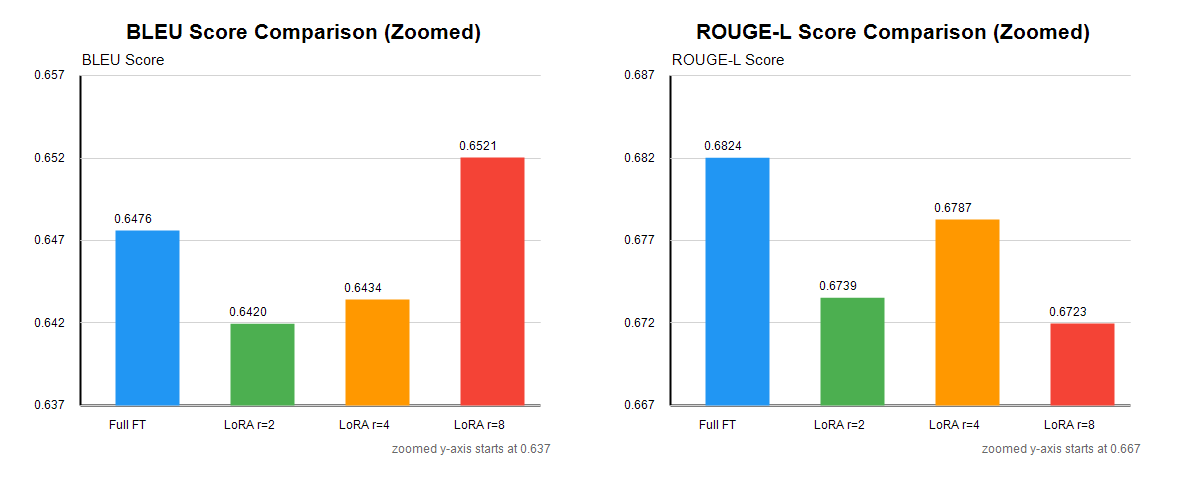
\includegraphics[width=0.93\linewidth]{../results/figures/metrics_comparison.png}
\caption{Zoomed comparison of BLEU and ROUGE-L across full fine-tuning and LoRA ranks.}
\end{figure}

\section{4. Results and Analysis}
Our results support the qualitative conclusion of the LoRA paper: low-rank adaptation achieved nearly the same generation quality as full fine-tuning while training far fewer parameters. The strongest parameter-efficiency comparison is LoRA $r=4$, which trained only 147,456 parameters, or 0.1184\% of the model, while reaching BLEU 64.34 and ROUGE-L 67.87. LoRA $r=8$ trained 294,912 parameters, or 0.2364\%, and slightly exceeded full fine-tuning on BLEU by 0.45 points. Full fine-tuning remained best on ROUGE-L, with 68.24 versus LoRA $r=4$ at 67.87 and LoRA $r=8$ at 67.23.

We do not interpret the LoRA $r=8$ BLEU result as proof that LoRA is generally better than full fine-tuning. The margin is small and likely within run-to-run variation. It is plausible because BLEU rewards exact n-gram overlap; a constrained LoRA model may produce more template-like generations that score well under BLEU, while full fine-tuning can change the model more broadly and may need a separately tuned learning rate. The more robust takeaway is that all LoRA variants were close to full fine-tuning despite training between roughly 400x and 1,688x fewer parameters.

The main discrepancy from the original paper is absolute score and model scale. Hu et al. used GPT-2 Medium and Large and reported means over multiple random seeds; we used GPT-2 Small and a single run per configuration because of compute limits. We also evaluated only BLEU and ROUGE-L, not NIST, METEOR, or CIDEr. These choices make our experiment a reasonable small-scale re-implementation rather than an exact reproduction. Still, the pattern matches Table 3: adapting only a small low-rank subspace of attention projections is enough to recover most of full fine-tuning's downstream performance.

\section{5. Reflections}
The main implementation lesson was that LoRA is conceptually simple but easy to get subtly wrong inside real model code. GPT-2's fused \texttt{c\_attn} layer required special handling because query, key, and value are not separate PyTorch \texttt{Linear} modules. Freezing behavior also needed explicit testing; otherwise, a run can look like LoRA while accidentally training base parameters.

The experimental lesson was that parameter-efficient fine-tuning should be evaluated as a tradeoff, not only by the best metric value. Full fine-tuning had much lower training loss, but LoRA produced similar test BLEU/ROUGE-L with a tiny trainable footprint. Given more time, we would run at least three random seeds, tune learning rates separately for full fine-tuning and each LoRA rank, report confidence intervals, and add METEOR/CIDEr to better match Table 3. We would also test LoRA on MLP projections and compare against adapters or prefix tuning to broaden the reproduction beyond full fine-tuning versus LoRA.

\section{6. References}
\small
Hu, E. J., Shen, Y., Wallis, P., Allen-Zhu, Z., Li, Y., Wang, S., Wang, L., and Chen, W. (2021). \textit{LoRA: Low-Rank Adaptation of Large Language Models}. arXiv:2106.09685.\\
Novikova, J., Dusek, O., and Rieser, V. (2017). \textit{The E2E Dataset: New Challenges for End-to-End Generation}. arXiv:1706.09254.\\
Radford, A. et al. (2019). \textit{Language Models are Unsupervised Multitask Learners}. OpenAI.\\
Wolf, T. et al. (2020). \textit{Transformers: State-of-the-Art Natural Language Processing}. EMNLP.\\
Bird, S., Klein, E., and Loper, E. (2009). \textit{Natural Language Processing with Python}. O'Reilly. Lin, C.-Y. (2004). ROUGE: A package for automatic evaluation of summaries.

\end{document}
